\chapter{データの収集と整理}

ClojureのコレクションはClojureでデータを集約する主要な手段であり、Clojureアプリケーションのすべてのレベルで使用されます。この章では、アプリケーション・データを作成、更新、およびアクセスするために、ドメイン・モデルの内側と外側の両方でコレクションを使用する方法に焦点を当てます。

異なるニーズに対して適切な種類のコレクションを選択し、作成する基本的なことから始めます。この選択は、主に、作成後にコレクションをどのように使用することを想定しているかによって行われます。

多くの場合、特別なコレクションや関数を使用して、一度にコレクションの大きな塊を更新することができます。また、マップ内のデータへのアクセスやシーケンシャルデータ内のアイテムの検索に関する懸念事項についても見ていきます。

最後に、これまで見てきた関数と連動するカスタムコレクションを作成する方法について見ていきます。これは高度なテクニックですが、特定のアプリケーションに合わせたデータ構造を作成するのに便利な方法です。


\section{正しいコレクションの選択}

Clojureは少数のコレクションを提供しており、事実上すべてのアプリケーションのニーズに合わせて組み合わせて使用されます。Clojureの4つの主要なコレクション、リスト、ベクター、セット、マップの基本はすでにご存知でしょう。

使用する正しいコレクションを選択するとき、私たちは手元のデータの特性と、コレクションに呼び出すと予想される操作によって導かれます。Clojureコレクション関数は、しばしば実装者が満たさなければならない性能制約を指定します。

キーから値への関連付けが必要な場合、マップは明白な選択です。ドメイン・モデルでは、エンティティ・ホルダーとして、つまり、エンティティ・フィールドと値の間の関連付けとして、マップを使用することを検討しました。また、Modeling Relationshipsでは、マップを識別子からエンティティへのインデックスとして使用しました。get関数を使ってキーに基づいた値を調べたいときは、いつでもマップが必要だ。

Clojureのセットは数学的なセットとして動作し、順序付けされない、重複を許さないという重要な特性を持ちます。セットは主に、contains? や get を使ってセットが値を含むかどうかを素早くチェックする必要があるような状況で使われます。

他のほとんどのデータは、本質的にシーケンシャルです。Clojureはシーケンシャルなデータ構造として、listとvectorを提供します。次に、それらの選択方法について見てみましょう。

\subsection{シーケンシャルコレクション}

シーケンシャルデータとは、順番に並んだ一連の値のことである。シーケンシャルデータでは、データの追加と削除を行う場所と、インデックス付きアクセス(シーケンシャルコレクション内の位置から要素を探せるかどうか)が重要な検討事項となります。

Clojureのリストは、各セルが値と次のセルへの参照を含むリンクリストデータ構造として実装されています。リストでは、既存のリストを指す新しいセルを作成し、それをリストの先頭にすることで、チェーンの先頭に新しいリンクを追加することは簡単です。これに対して、リストの末尾に要素を追加する場合は、新しいセルを追加する前にリスト全体を走査する必要がある。

リストが最適なケースとして、スタック(ビュッフェの皿の積み重ねのようなもの)が必要な場合がある。スタックは、データ構造(ツリーやグラフ)を横断するときに、どこにいたかを覚えておく必要がある場合に便利である。要素は、\texttt{cons} を介してスタックの一番上に押し出される。また、(\texttt{peek} で)先頭の値を見たり、(\texttt{pop} で)スタックの先頭の要素を削除したりすることもできる。

Clojure ベクターは、配列と使い方を比較することができ、その要素へのインデックス付きアクセスを提供します。ベクターは、コレクションの最初ではなく、最後に成長するように設計されています。

\texttt{conj} のような Clojure の操作は自然な挿入ポイントで要素を追加します--リストの場合は最初で、ベクターの場合は最後です。多くの新しいClojure開発者は、1つの操作が異なるデータ構造に対して異なる動作をすることに戸惑いを覚えます。しかし、\texttt{conj}は各データ構造に最適な場所で効率的に要素を追加するように設計されています。
 
第1章「ドメインのモデル化」のレシピの手順で、コレクションを選択することを考えてみましょう。ユーザーがステップを挿入したときの順序を保持したいのであれば、 順番に追加していくような動作をさせるために vector を使用するのが最も理にかなっています。また、レシピの指示で何かを行う必要がある場合、インデックスでステップを検索することが有用であると思われます。

これで、どのシーケンシャル・コレクションを使うか、ある程度決まったと思います。シーケンシャルコレクションは、挿入順序を保持するので便利です(挿入ポイントに依存します)。Clojureのセットとマップは順不同ですが、Clojureはこれが重要な場合のためにソートされたセットとマップを提供します。

\subsection{ソートされたコレクション}

ソートされたセットやマップを使用すると、データが追加されたときにセットやマップ全体で維持したい順序を指定することができます。

私たちのレシピアプリケーションでは、Authorsのインデックスを配信できるようにしたいと思います。Authorsは一意であり、これはセットを使用することを意味します。セットでは、自動的に重複が削除されます。Authorsのインデックスをアルファベット順で保持したい。

ソートされたセットはコンパレータ関数を使用して、要素のペアのソート順を決定します。コンパレータ関数は要素のペアに適用され、最初の要素がコレクション内の2番目の要素よりも低く、同じ、または高くソートされるべきかを示すために、負の整数、ゼロ、または正の整数を返します。

Clojureは、文字列のアルファベット順、数値の昇順など、一般的なデータ型のための「自然な」ソート順を与えるデフォルトのコンパレータ(比較関数で実装)を提供します。デフォルトのコンパレータは、常に\texttt{nil}を他の値よりも低くソートします。ソートされたマップでは、コンパレータはマップのキーに適用され、値には適用されません。

ソートされたセットとマップのカスタムコンパレータを実装する際の一般的な落とし穴は、2つの要素が同じと比較された場合、コレクションの重複削除プロパティのため、1つだけが保持され、もう1つが削除されることです。

たとえば、著者エンティティのカスタムコンパレータの最初の実装では、姓のみを使用する場合があります。

\begin{lstlisting}[numbers=none]
user> (defn compare-authors-badly [s1 s2]
        (compare (:lname s1) (:lname s2)))
#'user/compare-authors-badly
user> (sorted-set-by compare-authors-badly
        {:fname "Jeff" :lname "Smith"}
        {:fname "Bill" :lname "Smith"})
#{{:lname "Smith", :fname "Jeff"}}
\end{lstlisting}

\texttt{compare-authors-badly}は\texttt{lname}フィールドのみに基づいて同等性を定義しているため、2つのauthorマップはセットによって同一とみなされ、重複が削除されます。2つの要素が同じ値を持つ場合にのみ、等しいものとして比較されることを保証することが重要です。これを行う1つの方法は、まず以前のように姓でソートし、次にエンティティの他の各フィールド(ここではファーストネーム)を比較して同値を解除することです。

\begin{lstlisting}[numbers=none]
user> (defn compare-authors [s1 s2]
        (let [c (compare (:lname s1) (:lname s2))]
          (if (zero? c)
            (compare (:fname s1) (:fname s2))
            c)))
#'user/compare-authors
user> (sorted-set-by compare-authors
        {:fname "Jeff" :lname "Smith"}
        {:fname "Bill" :lname "Smith"})
#{{:lname "Smith", :fname "Bill"}
  {:lname "Smith", :fname "Jeff"}}
\end{lstlisting}

この関数は2つのフィールドだけを持つエンティティを比較しますが、エンティティのフィールドをカスタムオーダーで考慮するコンパレータをより簡潔に実装するための一般的なパターンも存在します。このパターンは、関数のコレクションを受け取り、入力にすべての関数を適用する新しい関数を作成し、結果のベクトルを返す、気の遠くなるような\texttt{juxt}関数に依存しています。

\texttt{juxt}を使うと、一連のキーワードをゲッター関数のように適用して、比較に適したフィールド値の順序付きシーケンスを生成することができます。

つまり、\texttt{(juxt :lname :fname)} はエンティティに適用して \texttt{["Smith" "Jeff"]} のようなベクトルを生成することができる関数を生成するのです。そして、デフォルトの比較関数を使用して、これらのフィールドベクトルを自然な順序(左から右へ)で比較することができます。

これをもとに構築してみよう。\texttt{compare-authors}の中にローカルの\texttt{project-author}関数を作成し、各authorフィールドに\texttt{juxt}を適用して比較用のベクトルを返します。

\begin{lstlisting}[numbers=none]
user> (defn compare-author [s1 s2]
        (letfn [(project-author [author]
                  ((juxt :lname :fname) author))]
          (compare (project-author s1) (project-author s2))))
#'user/compare-authors
user> (sorted-set-by compare-author
        {:fname "Jeff" :lname "Smith"}
        {:fname "Bill" :lname "Smith"})
#{{:lname "Smith", :fname "Bill"}
  {:lname "Smith", :fname "Jeff"}}
\end{lstlisting}

これは、underspecificationの問題を回避するカスタムエンティティコンパレータを作成するための便利なテクニックを示しています。これらのコンパレータの作成に関する詳細は、Andy Fingerhut氏の有用なコンパレータ・ガイドを参照してください。

さて、仕事に最適なコレクションを選択して作成する方法を検討したので、要素が追加、更新、削除されたときに、それらのコレクションを更新する最適な方法を検討しましょう。

 % Choosing the Right Collection
\section{コレクションを更新する}

私たちのアプリケーションは、新しい情報を受け取り、既存の情報を更新し、不要になった情報を削除するなど、常に外部と通信しています。しかし、これはClojureのイミュータブルなコア・コレクションと相反するように思えます。

Clojureでは、変化は常に純粋な関数をイミュータブルな値に適用し、その結果新しいイミュータブルな値が得られるというモデルになっています。言語学的なごまかしを避けるため、この変更手段を説明するために、単純な更新という言葉を使うことにします。

コレクションをイミュータブルに定義することには、多くの利点がある。まず、同時実行スレッドでは、値への参照ではなく、値の受け渡しが可能になる。これにより、他のスレッドによってデータが予測不可能に変更されることがない。第二に、ドメインロジックを状態管理機能から分離し、並行処理に関する問題をドメインデータや関数からきれいに分離します。

シーケンシャルなデータで発生する特殊なケースとして、キューのようにデータを更新する必要があります(先入れ先出し処理とも呼ばれる)。

\subsection{先入先出の処理}

ランチカウンターで、店員から注文が来ることを想像してください。公平性を保つために、注文は受け取った順に処理されることが期待されている - 先入れ先出し (FIFO) 処理。

Clojureでランチ・カウンターをモデル化するには、保留中のランチ・オーダーを保持するためのコレクションが必要です。ランチ・オーダーは時間的に自然な順序を持つので、リストやベクターのような連続したコレクションが必要なことが分かっています。ベクターを試してみましょう。

\begin{lstlisting}[numbers=none]
(defn new-orders [] [])

(defn add-order [orders order]
  (conj orders order))

(defn cook-order [orders]
  (cook (first orders)) (rest orders))
\end{lstlisting}

\texttt{add-order}関数は、\texttt{orders}の末尾に新しい\texttt{order}を追加しているので、vectorとしては効率的です。しかし、\texttt{orders}ベクターに対して\texttt{rest}を呼び出すのは非効率的です。これは、最初の要素以外のすべてを含むシーケンス(ベクターではない)を作成し、それを返します。もしベクターコレクション型を維持したければ、新しいベクターを構築し、そこにシーケンス要素を追加し直す必要があります;このすべてが高価です。

また、\texttt{orders}をリストで実装することもできる。\texttt{cook-order} のコードはそのままです。しかし、リンクされたリスト上で \texttt{rest} を呼び出すと効率的なので、ベクターで起こったパフォーマンスの問題に対処しています。しかし、\texttt{add-order}では新たな問題が発生しました。

\begin{lstlisting}[numbers=none]
(defn new-orders [] '())

(defn add-order [orders order]
  (concat orders (list order)))
\end{lstlisting}

リストの末尾にオブジェクトを追加する場合、リスト全体を走査して最後の要素を見つけ、新しいポインタを追加する必要があります。リストは先頭でのみ、ベクターは末尾でのみ効率的に追加と削除を行います。しかし、最後に追加し、最初に削除するコレクションが必要である。このニーズに応えるのが、次の図に示すようなキュー(待ち行列)です。

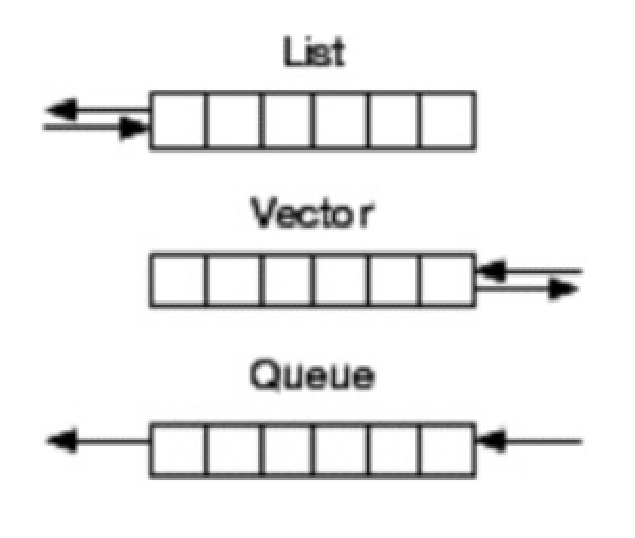
\includegraphics[width=5cm]{fig_02_001.eps}


他のすべてのコアコレクションと同様に、キューは不変の永続的なコレクションであり、リストやベクトルを扱うのと同じ関数をすべてサポートしています。以下は、ランチカウンターをキューで実装する方法です。

\begin{lstlisting}[numbers=none]
(def new-orders clojure.lang.PersistentQueue/EMPTY)

(defn add-order [orders order]
  (conj orders order))

(defn cook-order [orders]
  (cook (peek orders))
  (pop orders))
\end{lstlisting}

Clojureはリテラルなキューの構文やコンストラクタを提供しません。新しいキューを作成するには、静的な空のインスタンス \texttt{clojure.lang.PersistentQueue/EMPTY} で開始します。\texttt{add-order}では、vectorのように最後に新しい要素を追加するために\texttt{conj}を使用するだけです。\texttt{cook-order}では、最初の順序を見るために\texttt{peek}を使い、最初の順序以外を返すために\texttt{pop}を使います。

待ち行列の実装は、順序の追加と、待ち行列に入れられた順序での順序の削除の両方において効率的です。これは、この仕事に適したツールです。

次に、コレクションにデータを追加する処理を最適化する方法を考えてみましょう。


\subsection{一括インポート}

Clojureの永続的なコレクションは、イミュータブルです。効率化のために、\texttt{conj}や\texttt{assoc}のような関数で要素を追加すると、新しい不変の構造が作成されますが、その前と後のバージョンは通常そのデータの多くを共有します。コレクションは不変なので、これは安全に実行でき、データをコピーするよりもはるかに高速です。しかし、Clojureは制御されたコンテキストでミュータビリティを活用することで、より効率的にコレクションを埋める方法があります。

典型的なケースは、カタログアイテムのインポートです。アプリケーションが記録システムに直接アクセスできない場合、そのシステムからのエクスポートは、開始時にアプリケーションにインポートすることができます。カタログが変更されると、定期的な更新が必要になることは容易に想像できる。大規模なカタログの場合、その処理には時間がかかることがあります。

アプリケーションの起動時に呼び出される典型的なインポートを考えてみましょう。


\begin{lstlisting}[numbers=none]

\end{lstlisting}








\begin{lstlisting}[numbers=none]

\end{lstlisting}





 % Updating Collections
\section{コレクションにアクセスする}

コレクションの目的はデータを保存することですが、データをコレクションから取り出せてこそ、コレクションは役に立ちます。まず、キーによる索引検索をサポートするコレクションを考えてみましょう。

\subsection{インデックス付きアクセス}

Clojureで提供されるインデックス付きコレクションは、マップとベクターの2つです。ベクターは0ベースのインデックスを使用し、インデックスから要素への連想コレクションとして扱われます。ドメインをモデリングしているときに見たレコードもマップインターフェースを実装しており、インデックス付きコレクションとして扱うことができます。

インデックス付きコレクションは3つのメソッドで検索をサポートする。1つ目は、コレクションとキーを指定して\texttt{get}関数を呼び出す方法である。2つ目は、コレクションそのものをキーとともに呼び出す方法である。3つ目は、コレクションをキーワードやシンボルで呼び出す方法です。以下は、3つの方法の例である。

\begin{lstlisting}[numbers=none]
(def earth {:name "Earth" :moons 1})

(get earth :name) ;; (1) using get
(earth :name) ;; (2) invoking the map
(:name earth) ;; (3) invoking the keyword key
\end{lstlisting}

これらの3つの方法はすべて典型的なClojureプログラムで使用されますが、それぞれトレードオフが異なり、状況によって好まれる方法が異なります。

エンティティ(マップまたはレコード)については、関数としてキーワードを呼び出すことが好ましい方法であり、このスタイルの検索は広く使用されています。関数としてのキーワードキーの使用は、他の関数を入力として受け取るClojureライブラリの多くの関数とうまく連動します。

マップがデータの定数ルックアップ・テーブルとして、またはキーから値への関数として使用されている場合、マップを関数として呼び出すのが一般的です。この呼び出しスタイルの欠点は、呼び出されるマップが\texttt{null}の可能性がある場合、\texttt{NullPointerException}が発生することです。このため、この呼び出しスタイルは、\texttt{def}を使用して、決して\texttt{null}にならない一定のグローバルマップを作成した場合によく見受けられます。レコードは呼び出すことができないので、この方法では呼び出すことができないことに注意してください。

何が起こっているのかが不明な場合は、\texttt{get}を直接呼び出すと便利です。例えば、マップを作成する関数が使われているとき、関数の戻り値がたまたまルックアップテーブルであった場合に呼び出すと混乱することがある。

例えば、ここにある \texttt{opposite-colors} 関数は、特定のパレットにある色と対照的な色のマッピングを返します。

\begin{lstlisting}[numbers=none]
(defn opposite-colors
  "Compute an opposite-color mapping for a given palette."
  [palette]
  ;; This function should compute the mapping for the palette and
  ;; return a map like this with many entries: {:magenta :green}
  )
\end{lstlisting}

それに対する呼びかけを紹介します。

\begin{lstlisting}[numbers=none]
((opposite-colors palette) :magenta) ;; ok, but confusing
(get (opposite-colors palette) :magenta) ;; less confusing
\end{lstlisting}

最初の呼び出しの例は \texttt{opposite-colors} が返すマップを直接呼び出していますが、多くの Clojure 読者はこの使い方につまずき、何が起こっているのか不思議に思ってから解決することでしょう。一般的に、式の右側で閉じ括弧を山ほど見ることはよくありますが、左側で同じことを見ることは比較的まれです。関数を呼び出して、その戻り値をすぐに呼び出すということはほとんどありません。

2番目の呼び出しの例では、代わりに明示的にget関数を使用しています。これは、読者に対して、\texttt{opposite-colors}から返される値がマップであることを強く知らせるものです。このコードでは、\texttt{opposite-colors}が\texttt{nil}を返す場合にも対応しており、その場合は\texttt{get}も\texttt{nil}を返します。

マップから単一の値を取り出すこれらの方法に加えて、時にはサブマップを取り出し、エントリーの部分的なセットを選択することが有用である。Clojureはこの目的のために\texttt{select-keys}関数を提供します。この関数は常にハッシュ・マップを返し、ソース・タイプ(レコード、ソート・マップなど)のマップは返しません。

もし、私たちが宇宙シミュレーションからデータのエクスポートを準備していたなら、最も重要なキーのうちのいくつかだけを選択して、情報の一部を省略した簡略化したエクスポートを提供することができます。

\begin{lstlisting}[numbers=none]
(defn export-planet
  [planet]
  (select-keys planet [:name :moons]))
\end{lstlisting}

エクスポートされる惑星は、単純なマップになります。\texttt{\{:name "Earth" :moons 1\}} というシンプルなマップになります。次に、シーケンシャルなデータ構造の中のものを探すことに目を向けましょう。

\subsection{逐次探索}

前節で扱ったマップは、ある値を効率的に一定時間で調べたいときに常に理想的な選択肢となる。同様に、セットも\texttt{contains?}関数を使って、あるセットが特定の値を含んでいるかどうかを素早くチェックすることができます。しかし、\texttt{contains?}関数はリストやベクトル内の値で項目を探すのには使えません。

順番に並んだコレクションが必要で、かつそのコレクションの中の値も見つける必要がある場合、コレクションを順番に検索して一致するものを見つける方法が必要です。この検索にかかる時間は、コレクションのサイズに比例することに注意する必要があります。

Clojureで見られる逐次探索の最も一般的なテクニックの1つは、some関数を使うことです。この関数はコレクションの各要素に対して述語を評価し、最初の論理的に真となる値(元の要素ではありません)を返します。これは単純な値のコレクションで最も便利です。

\begin{lstlisting}[numbers=none]
(def units [:lb :oz :kg])

(some #{:oz} units)
;;=> :oz
\end{lstlisting}

\texttt{some}と一緒に使われている述語は、1つの値を含むセットです。ここでは、前のセクションと同じコレクション呼び出しのスタイルを活用し、ユニットベクタの各要素を順番に持つ関数としてセットを呼び出しています。マッチングが成立すると、その値が返されます。結果は真理値として使用することができます。マッチしない場合は、\texttt{nil}が返される。

この目的のために\texttt{some}を使うことはよくあるが、論理的に偽である\texttt{nil}や\texttt{false}を探すという特殊なケースで破綻する。

論理的に偽の値の検索をサポートし、早期に終了する比較的効率的な線形探索の実装は以下のように定義できる。

\begin{lstlisting}[numbers=none]
(defn contains-val?
  [coll val]
  (reduce
    (fn [ret elem] (if (= val elem) (reduced true) ret))
    false coll))

(contains-val? units :oz)
;;=> true
\end{lstlisting}

\texttt{reduce}と\texttt{reduced}の使い方は、Reducing to a Valueで詳しく説明します。

Clojureが提供するコレクションをどのように活用するか決めたところで、独自のコレクションを構築する方法を検討することで、自分のアプリケーションに固有の問題を解決する方法も考えたいと思います。

 % Accessing Collections
\section{カスタムコレクションの構築}

Clojureのコレクションがどれもあなたの問題に適していない場合、あなた自身でロールバックする必要があるかもしれません。標準のコレクションと同様に、カスタム・コレクションはClojureコア・ライブラリでシームレスに使用できます。カスタム・コレクションを構築するには、Clojureが内部で使用するtraitインタフェースを実装するためにdeftypeを使用することが必要です。

\subsection{コレクションの特徴}

Clojureが使用できるコレクションを構築したい場合、Clojureがコレクションとどのように相互作用するかをより深く理解する必要があります。コレクションとシーケンスライブラリは、Clojureに含まれる特定の実装ではなく、主要な抽象化を定義する特質の一般的なセットに基づいています。Clojureのコレクション特質は、Javaインタフェースを使用して内部的に実装されています。

述語関数は、コレクション実装上のClojureコレクションの特徴の存在を検出するためにClojureで提供されます。述語関数は質問をし、ブール値の答えを返しますが、Clojureでは慣例的に名前に末尾の\texttt{?}をつけます。

Clojureの述語コレクション関数には、以下のようなものがあります。


\begin{itemize}
\item \texttt{counted?}--コレクションは一定時間内に数えることができるか?
\item \texttt{sequential?}--値が特定のトラバース可能な順序で格納されているか?
\item \texttt{associative?}--コレクションはキーと値の間の関連性を保存しているか?
\item \texttt{reversible?}--コレクションは可逆的か?
\item \texttt{sorted?}--コレクションはソートされた順序で管理されているか?
\end{itemize}

これらの特質は、以下のJavaインタフェースに対応している。\texttt{Counted}、Sequential、\texttt{Associative}、\texttt{Reversible}、\texttt{Sorted}です。その他の内部インターフェースは、コアコレクションインターフェースの構造や、パブリックコレクション関数の下で使われる主要なメソッドを定義している。

カスタムコレクションを構築するとき、実装したいClojure関数から、その関数をサポートするためにコレクションに必要な実装のJavaインタフェースまで、逆算する必要があります。

この図は、Clojure関数(右の列)からJavaメソッド(左の列)へのマッピングを提供します。各インターフェースに対する述語関数は、各Javaインターフェース名の下に記載されています。

\begin{figure}[h]
\centering
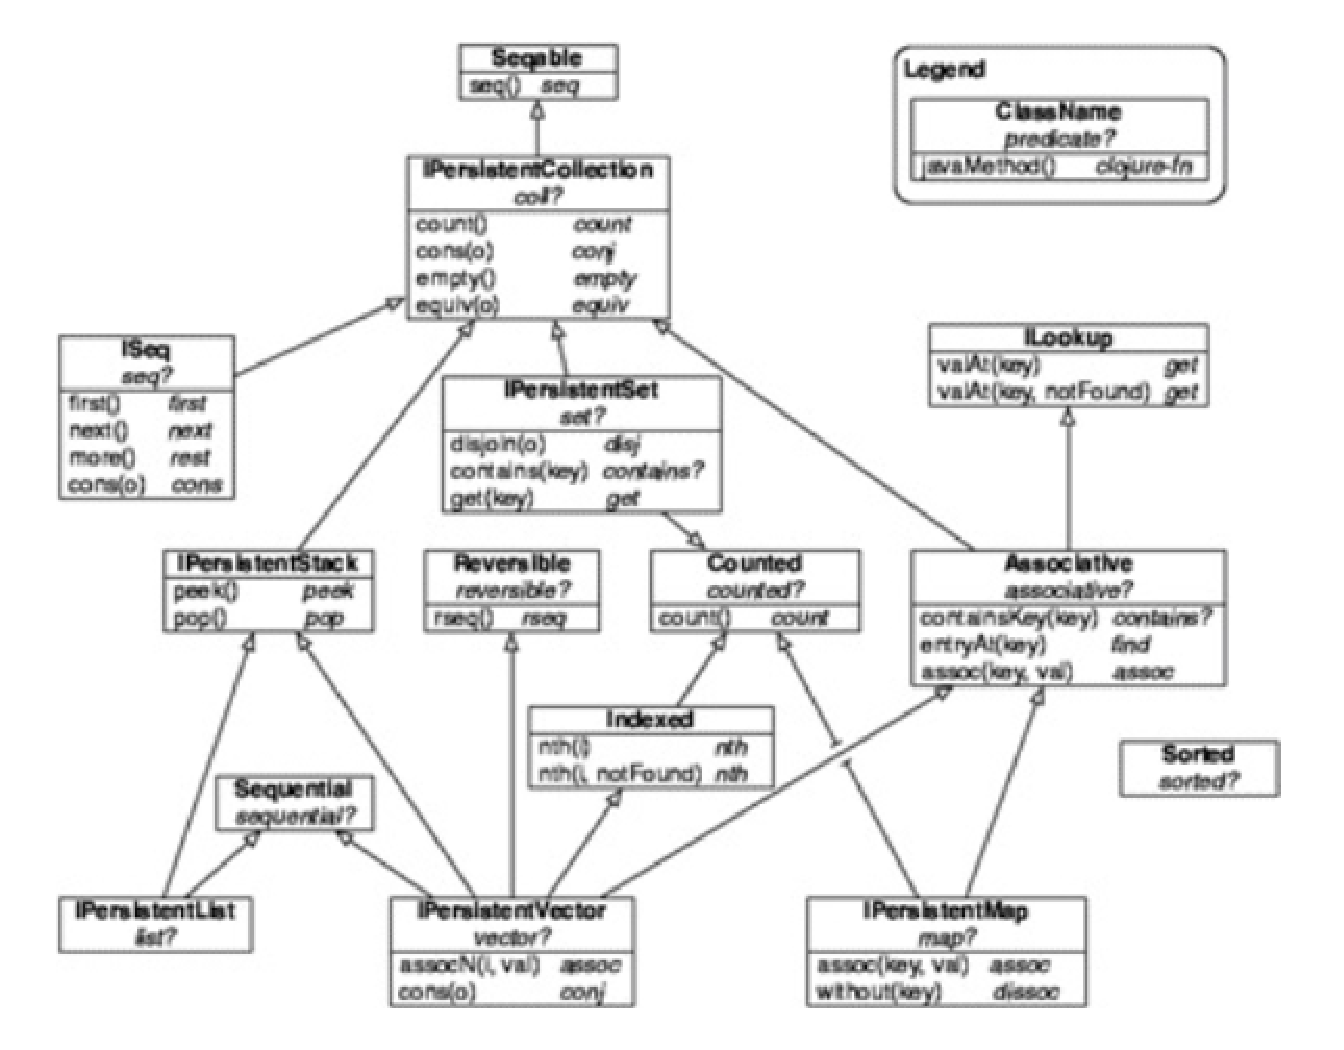
\includegraphics[width=8cm]{fig_02_002.eps}
\caption{Clojure関数とそれに対応するJavaメソッド}
\end{figure}

Clojureで意図した使用方法とマッピング図を用いて、目的を満たすカスタムコレクションを構築する方法を見てみましょう。

\subsection{deftypeでコレクションを作成する}

まず、このコレクションが何をする必要があるのかを考えてみましょう。a と b と呼ぶ 2 つの値を保持するカスタム \texttt{Pair} クラスを実装するつもりです。\texttt{Pair} 型は \texttt{seq}、\texttt{count}、\texttt{nth}、および \texttt{get} で動作するようにしたいと思います。図を見てみると、\texttt{Seqable}、\texttt{Counted}、\texttt{Indexed}、\texttt{ILookup}を実装する必要があることがわかります。

カスタムデータ構造を実装するには、\texttt{deftype}マクロを使用します。
これは\texttt{defrecord}に似ているが、より多くの機能を提供し、マップとの組み込みの類似性は少ない。例えば、\texttt{deftype}は\texttt{record}と同じように型とコンストラクタ関数を取得しますが、自動的にマップのように動作するわけではありません。\texttt{deftype}では、必要であればマップのように振舞うために適切なインタフェースを実装するのは我々の責任である。型はまた、他のClojure構成要素では利用できない、mutableフィールドやunsynchronizedフィールドのような特殊な機能のサポートを持っています。

\texttt{Pair}が\texttt{deftype}としてどのように見えるか見てみましょう。

\begin{lstlisting}[numbers=none]
(ns ch2.pair
  (import [clojure.lang Counted Indexed ILookup Seqable]))

(deftype Pair [a b]
  Seqable
  (seq [_] (seq [a b]))

  Counted
  (count [_] 2)

  Indexed
  (nth [_ i]
    (case i
      0 a
      1 b
      (throw (IllegalArgumentException.))))
  (nth [this i _] (nth this i))

  ILookup
  (valAt [_ k _]
    (case k
      0 a
      1 b
      (throw (IllegalArgumentException.))))
  (valAt [this k] (.valAt this k nil)))
\end{lstlisting}

\texttt{deftype}の内部では、実装される各インターフェースをリストアップし、次にメソッドの実装を提供します。

これでREPLから\texttt{Pair}型を利用することができるようになりました。

\begin{lstlisting}[numbers=none]
user> (use 'ch2.pair)
nil
user> (def p (->Pair :a :b))
#'user/p
user> (seq p)
(:a :b)
user> (count p)
2
user> (nth p 1)
:b
user> (get p 0)
:a
user> p
#object[ch2.pair.Pair 0x39b4cec7 "ch2.pair.Pair@39b4cec7"]
\end{lstlisting}

\texttt{p}を直接見ようとするまではうまくいっていたのですが、これから修正します。

\subsection{型のカスタム表示}

先ほど見たように、型にはクラス名と識別子を含むあらかじめ定義された表示フォーマットがあります。私たちの型の表示形式には、インスタンスデータが含まれるようにしたいのです。リーダーはClojure内部のコンポーネントで、文字列を読み込んでClojureデータを返します。理想的には、リーダーによって読むことができるフォームで私たちの型を表示したいです -- これはリテラル値として私たちに完全なラウンドトリップ能力を与えます。

表示装置は、カスタムプリンターを供給するフックを定義するマルチメソッドを持つオープンシステムです。考慮すべきは、\texttt{print-method}(ユーザのために表示するときに呼び出される)と\texttt{print-dup}(リーダーのために表示するときに呼び出される)の2つのフックである。例えば、Clojure文字列は、\texttt{print-method}では周囲の引用符なしで表示されますが、 \texttt{print-dup}では周囲の引用符で表示されます。

私たちの目的のために、私たちはどちらの場合でも同じようにペアタイプを表示したいので、単に\texttt{print-method}を呼び出すために\texttt{print-dup}を実装することにします。

\begin{lstlisting}[numbers=none]
(defmethod print-method Pair
  [pair ^Writer w]
  (.write w "#ch2.pair.Pair")
  (print-method (vec (seq pair)) w))

(defmethod print-dup Pair
  [pair w]
  (print-method pair w))
\end{lstlisting}

そのため、今回のプリンターでは、\texttt{Pair}データをベクターに変換し、既存のベクター用\texttt{print-method}に対応させることで簡略化しています。試してみましょう。

\begin{lstlisting}[numbers=none]
user> (use 'ch2.pair.print)
nil
user> (->Pair 1 2)
#ch2.pair.Pair[1 2]
user> #ch2.pair.Pair[3 4]
#ch2.pair.Pair[3 4]
\end{lstlisting}

Clojureリーダーはこの形式を使用してJavaオブジェクトを構築するため、今回表示する構文は特別に選択されました。フォーマットは\tex{#class\[args\]}です。前のコードでは、コンストラクタ・クラスの構文を REPL に置くと、リーダーはそれを \texttt{Pair} オブジェクトに読み込んで、プリンタは私たちの \texttt{print-method} プリンタを使用して結果のオブジェクトを表示します。

 % Building Custom Collections
\section{まとめ}

これで、ドメインモデルの内部と外部の両方でコレクションを使用して、エンティティと値の両方を収集する方法について完全に理解しました。Clojureアプリケーションのデータのほとんどは、ここで説明したコレクション以外から構築されていません。時折、特殊な考慮事項やパフォーマンスを最大化するために、独自のコレクションを構築することが有用であることが分かるでしょう。

第4章「状態、アイデンティティ、および変更」で状態をどのように管理することを期待するかについて、段階を踏んでいます。この章で説明した概念と同様に、状態管理は不変の値と純粋な変換関数の基礎に大きく依存しています。

しかし、まずはコレクションと関数に関する知識を活かして、データを処理する能力をどのように拡張するかに焦点を当てます。これまでは、主にコレクション・レベルで、単一の値やエンティティを変更してきました。次に、範囲を広げてシーケンスについて説明します。

シーケンスとは、リストやベクターなどのコレクションをシーケンシャルなデータ構造のように扱えるようにするための一般化表現です。Clojureのデータ変換機能のほとんどは、特定のコレクションに縛られることなく、このより一般的な抽象化の上に構築されています。Clojureのデータ変換関数は、強力で再利用可能なClojureアプリケーションを書くための重要な部分です。
 % Wrapping Up

     
    
         